Gibbsovo uzorkovanje pripada Monte Carlo Markovljevim \engl{Monte Carlo Markov Chain, MCMC} metodama. Markovljevim lancima modelira se bezmemorijski matematički sustav stanja i prijelaza između stanja \citep{kass1998markov}. Markovljev lanac je niz vrijednosti generiranih u procesu s Markovljevim svojstvom. Prema Markovljevom svojstvu međuovisnost postoji samo između susjednih vrijednosti, tj. vrijednost u Markovljevom lancu generira se samo na temelju prethodne vrijednosti, zbog čega se nazivaju bezmemorijskim. 

Gibbsovo uzorkovanje zadovoljava obilježja Monte Carlo metoda i Markovljevih lanaca. Metoda generira niz uzoraka, gdje su generirani susjedi međusobno zavisni (korelirani). Početni uzorci \engl{burn out period} Gibbsovog uzorkovanja se često zanemaruju jer ne predstavljaju ciljanu distribuciju.


%%KRAJ UVODA

\section{Pretpostavke}

Distribucija iz koje je potrebno uzorkovati je "posebna", jer nije moguće uzorkovati izravno. Izračun vjerojatnosti sunčanog ili kišovitog vremena tijekom sutrašnjeg dana proces je koji je moguće procijeniti Gibbsovim uzorkovanjem. No, informacije koje su potrebne za Gibbsovo uzorkovanje su informacije o uvjetnim distribucijama vjerojatnosti sunčanog, odnosno kišovitog vremena. Potrebno je poznavati vjerojatnosti o vremenu temeljem današnjeg vremena. Odnosno, ukoliko nas zanimaju $P(sutra = ki$š$a)$ i $P(sutra = sunce)$, potrebno je poznavati vjerojatnosti:
\begin{itemize}
\item $P(sutra = ki$š$a | danas = ki$š$a)$
\item $P(sutra = ki$š$a | danas = sunce)$
\item $P(sutra = sunce | danas = ki$š$a)$
\item $P(sutra = sunce | danas = sunce)$
\end{itemize}



\chapter{Monte Carlo metode}

\section{Povijest}

Monte Carlo metode obuhvaćaju računalne modele zasnovane na stohastičkoj matematici, točnije, uporabi nasumičnih brojeva u izračunima. Moderne Monte Carlo metode osmislio je Stanislaw Ulam \citep{kass1998markov}, a ime su dobile po omiljenom odredištu zabave Ulamovog ujaka -- Monte Carlo kockarnicama. Originalno su zamišljene kako bi pomogle pri difuziji neutrona. Svrha Monte Carlo metoda bila je izraditi umjetno stvoriti nasumičan proces bez mogućnosti upravljanja njime. John von Neumann, slavni znanstvenik, uvidio je potencijal Monte Carlo metode i implementirao ih na računalu ENIAC. Intenzivnija primjena Monte Carlo metoda počela je s pojavom snažnijih računala. 

\section{Mehanizam}

Monte Carlo metode pokušavaju oponašati slučajne procese u prirodi (npr. bacanje novčića). Na taj način pokušavaju se predvidjeti svi mogući ishodi i vjerojatnosti događaja unutar okvira zadanog procesa. 

Monte Carlo metoda je probabilistički računalni algoritam koji pokušava predvidjeti sve moguće ishode i vjerojatnosti procesa na koji je primijenjen. Temelji se na slučajnim varijablama, koje je potrebno zadati u obliku funkcije gustoće \citep{gilks1996markov}. Na temelju funkcija gustoće $P(x)$ Monte Carlo metodama moguće je riješiti probleme:
\begin{itemize}
\item generiranja $R$ uzoraka $\{x^{(r)}\}_{r=1}^{R}$ iz $P(x)$,
\item izračun očekivanja funkcija s distribucije $P(x)$.
\end{itemize}


Monte Carlo metodama se simuliraju sustavi s mnogo neizvjesnosti. Pokazale su se iznimno učinkovite prilikom modeliranja složenih vjerojatnosti i strategija odlučivanja kojima nije moguće upravljati, ili ih je iznimno teško ili zahtjevno izgraditi. Izračun osiguranja, modeliranje kreditnih rizika u financijskim institucijama, rekonstrukcija eksplozija samo su neki primjeri u kojima se koriste Monte Carlo metode, zbog činjenice da je navedene procese u stvarnosti teško simulirati i pratiti. 

U Monte Carlo analizama potrebno je definirati distribucije vjerojatnosti slučajnih varijabli. Markovljevim lancima moguće je modelirati međuovisnost, što nije moguće Monte Carlo metodama. Ukoliko je potrebno dobiti uzorke iz aposteriori distribucije vjerojatnosti, Markovljevim lancima moguće je uzastopno uzorkovati dok uzorkovanje ne postane stabilan proces. Tada je moguće dobiti nezavisne uzorke iz aposteriori distribucije vjerojatnosti. 

Monte Carlo integracija pripada Monte Carlo metodama, a služi za izračun integrala. 

Monte Carlo metode imaju svojstvo crne kutije \engl{black box}. Njima je moguće dobiti odgovore na razna pitanja procjene vjerojatnosti, kao: kolika je vjerojatnost kiše sutra, kolika je vjerojatnost da će Googleova dionica izgubiti na vrijednosti, kolika je vjerojatnost da će klijent vratiti kredit \dots No, nije moguće saznati koji su razlozi na temelju kojih je dobivena određena vjerojatnost. 

\chapter{Markovljev lanac}

Markovljeve lance inicijalno je predstavio ruski znanstvenik Andrey Markov 1912. godine. Markov je pokušao modelirati slavno remek djelo Aleksandra Puškina \textit{Jevgenij Onjegin}. Cilj modela bio je predviđanje idućih slova temeljem trenutnih. Markovljeva ideja je po prvi puta predstavila koncepte zavisne varijable i uvjetne vjerojatnosti.

\begin{figure}
\centering
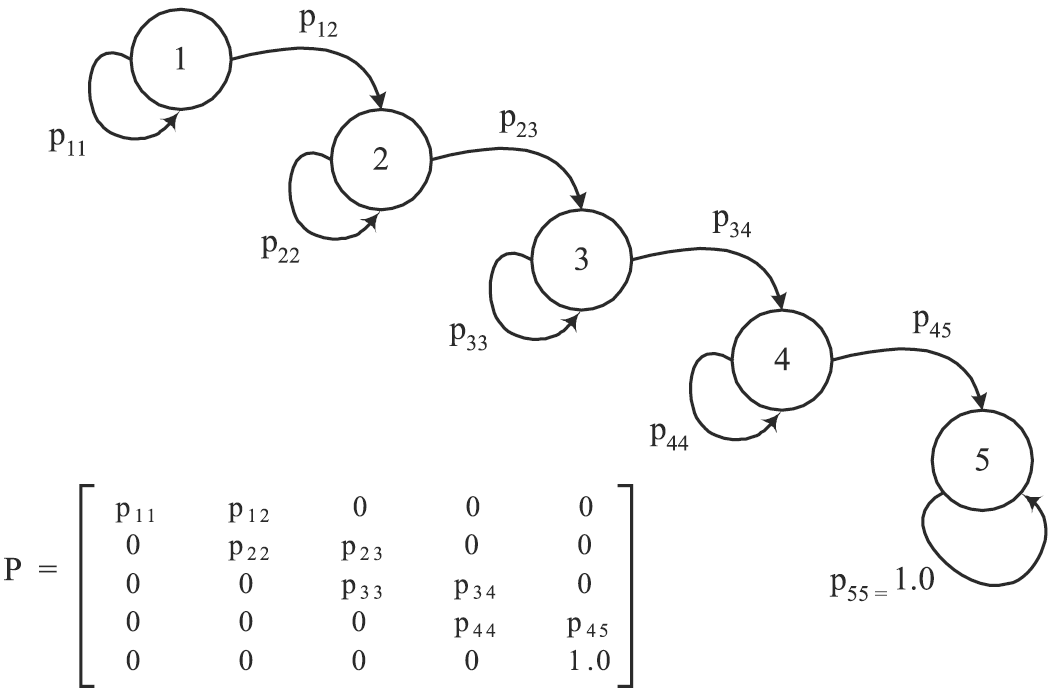
\includegraphics[scale=1]{markov_chain_example.png}
\caption{Primjer Markovljevog lanca. Preuzeto iz \citep{wirahadikusumah2003application}.}
\label{fig:markov_example}
\end{figure}

Markovljevi lanci se, također, primjenjuju nad širokim spektrom problema. Koriste se za modeliranje događaja i njihovih vjerojatnosti kada nije potrebno pamtiti prošle događaje. Markovljevi lanci sastoje se od niza stanja i vjerojatnosti prijelaza između stanja. Primjer Markovljevog lanca prikazan je slikom \ref{fig:markov_example}. Na slici je vidljivo pet stanja označenim brojevima u krugovima, jednosmjernih strelica kojima se označavaju mogućih prijelazi te matrica prijelaza $P$, matrični zapis Markovljevog lanca. Markovljev lanac ima oblik usmjerenog grafa. Stanja na burzama dionica, vremenska prognoza, prepoznavanje govora su neke od problema koji se često modeliraju Markovljevim 
lancima. 

Markovljevi lanci pretpostavljaju kako je sustav koji se modeliraju stabilan. U praksi, to često nije tako. Kompleksni sustavi, kao što su burze dionica,  sastoje se od pravilnosti i šuma. No, često moguće procijeniti jesu li vjerojatnosti dobivene danas relevantne za nekoliko godina.

\chapter{Gibbsovo uzorkovanje}

Gibbsovo uzorkovanje je dobilo ime po Josiahu Willardu Gibbsu, američkom znanstveniku 19. stoljeća koji je izumio Gibbsova nasumična polja. Stuart i Donald Geman su prvi puta opisali postupak Gibbsovog uzorkovanja \citep{geman1984stochastic}. Braća Geman bavili su se izradom modela za analizu slike. Gibbsovo uzorkovanje u njihovom radu je poseban slučaj Metropolis-Hastings algoritma \citep{metropolis1953equation}. \citep{gelfand1990sampling} su pokazali potencijalne primjene Gibbsovog uzorkovanja prilikom rješavanja velikog broja statističkih problema.

Gibbsovo uzorkovanje koristi Monte Carlo tehnike za procjenu vjerojatnosti u modelu zasnovanom na Markovljevom lancu. Prema tome, Gibbsovo uzorkovanje primjenjuje se u kompleksnim sustavima visokog stupnja entropije, gdje pretpostavljamo da iduće stanje ovisi samo o trenutnom stanju. Najčešće se koristi za izračune vrijednosti određenih integrala, posebice u višedimenzionalnim slučajevima. 

Metropolis Hastings algoritam sličan je algoritmu Gibbsovog uzorkovanja. Metropolis Hastings algoritam ne donosi odluke temeljem svih uvjetnih distribucija vjerojatnosti, već donosi odluku o prihvaćanju ili odbijanju učinjenog koraka (odbijanje vodi u prethodni korak). 

Ako je moguće dobiti nezavisne uzorke izravno iz distribucije, dovoljno je koristiti Monte Carlo mehanizme. Ukoliko su poznate samo uvjetne vjerojatnosti, a potrebno je uzorkovati iz zajedničke distribucije vjerojatnosti nužno je koristiti Metropolis Hastings algoritam ili Gibbsovo uzorkovanje. Gibbsovo uzkorkovanje daje uzorak za svaki korak, ali zahtjeva potpunu informaciju o uvjetnim distribucijama vjerojatnosti, što Metropolis Hastings algoritam ne zahtjeva, već odbacuje dobivene uzorke ukoliko su dobiveni na temelju izrazito niske vjerojatnosti. 

Gibbsovo uzorkovanje neće uvijek konvergirati. 